\documentclass{beamer}

% Choose how your presentation looks.
%
% For more themes, color themes and font themes, see:
% http://deic.uab.es/~iblanes/beamer_gallery/index_by_theme.html
%
\mode<presentation>
{
  \usetheme{Darmstadt}      % or try Darmstadt, Madrid, Warsaw, ...
  \usecolortheme{beaver} % or try albatross, beaver, crane, ...
  \usefonttheme{serif}  % or try serif, structurebold, ...
  \setbeamertemplate{navigation symbols}{}
  \setbeamertemplate{caption}[numbered]
} 

\usepackage[english]{babel}
\usepackage[utf8x]{inputenc}
\title[Background and Literature]{Enhance Speech Text Alignment For Prosody Modeling And Prediction In TTS}
\author{Aghilas Sini}
\institute{Université de Rennes 1}
\date{13/01/2017}

\setbeamertemplate{bibliography item}{}

%remove line breaks
\setbeamertemplate{bibliography entry title}{}
\setbeamertemplate{bibliography entry location}{}
\setbeamertemplate{bibliography entry note}{}



\begin{document}

%============================================================%
% Title Frame 
%============================================================%
\begin{frame}
  \titlepage
\end{frame}



\section{Speech To Text Alignment}
%============================================================%
%
%============================================================%
\subsection{Overview}
\begin{frame}{Forced Alignment}

\begin{figure}[!h]
\begin{center}

   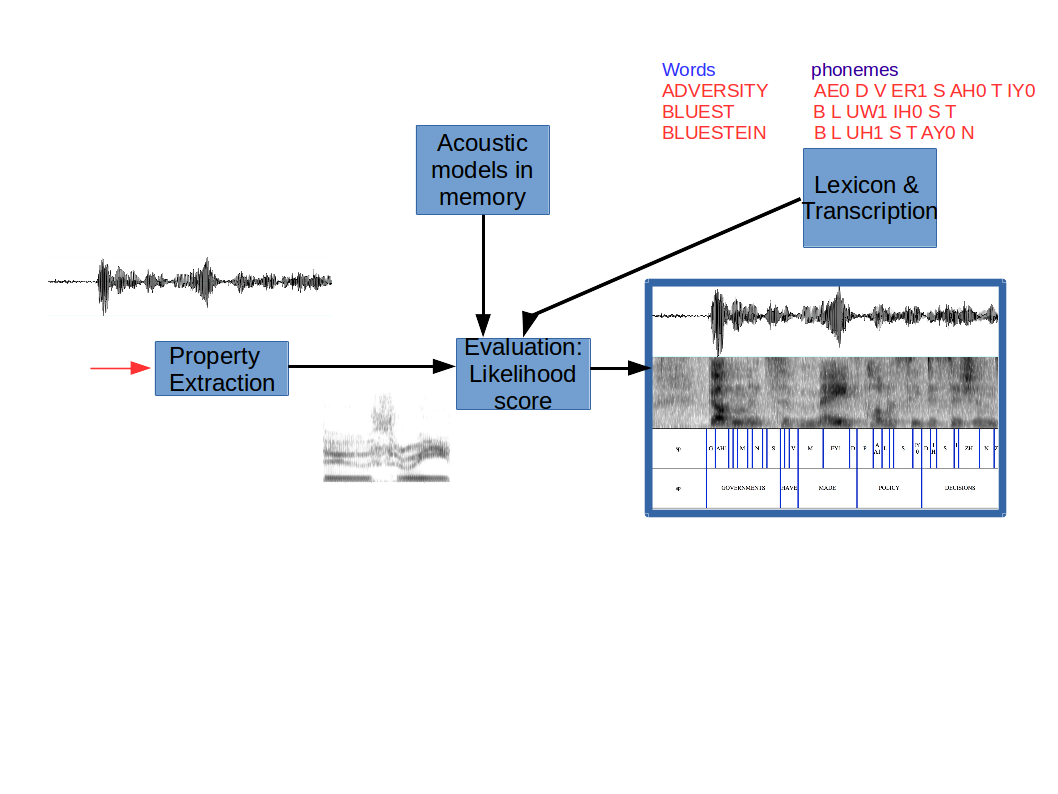
\includegraphics[scale=0.38]{/home/asini/Workspace/TexTemplates/asImages/forced_alignment.png}
\caption{Forced Alignment System}
\end{center}

\end{figure}
	
	
	
	
\end{frame}
%============================================================%
%
%============================================================%
\subsection{Adapting The Default Acoustic Model}
\begin{frame}{Why?}
	\begin{itemize}
		\item Adapt data properties (words, phonemes ... )
		\item Voice characteristics.
		\item Take account recording environment (robustness)
		\item Accurate boundaries (words, silences ... )
	\end{itemize}

\end{frame}

%============================================================%
%
%============================================================%
\subsection{Problems In Text Processing }
\begin{frame}{Text Pre-processing(Classical Problems)}
	Since the texts are  too long
		\begin{itemize}
			\item sentence end detection (choice should be done..)
			\item Dealing with abbreviations.
			\item Recognizing Acronyms and URLs.
			\item Processing numbers
			\item Dealing with idioms and proper name.
		\end{itemize}
	 Note : I'm trying to solve the above problems using different existing toolkit, this introduce another issues... And I think that we need manual checking ... 
	 \end{frame}
%============================================================%
%
%============================================================%
\subsection{NEB Corpus }
\begin{frame}{Gaëlle Vidal Work to Complete!!}
\begin{figure}
	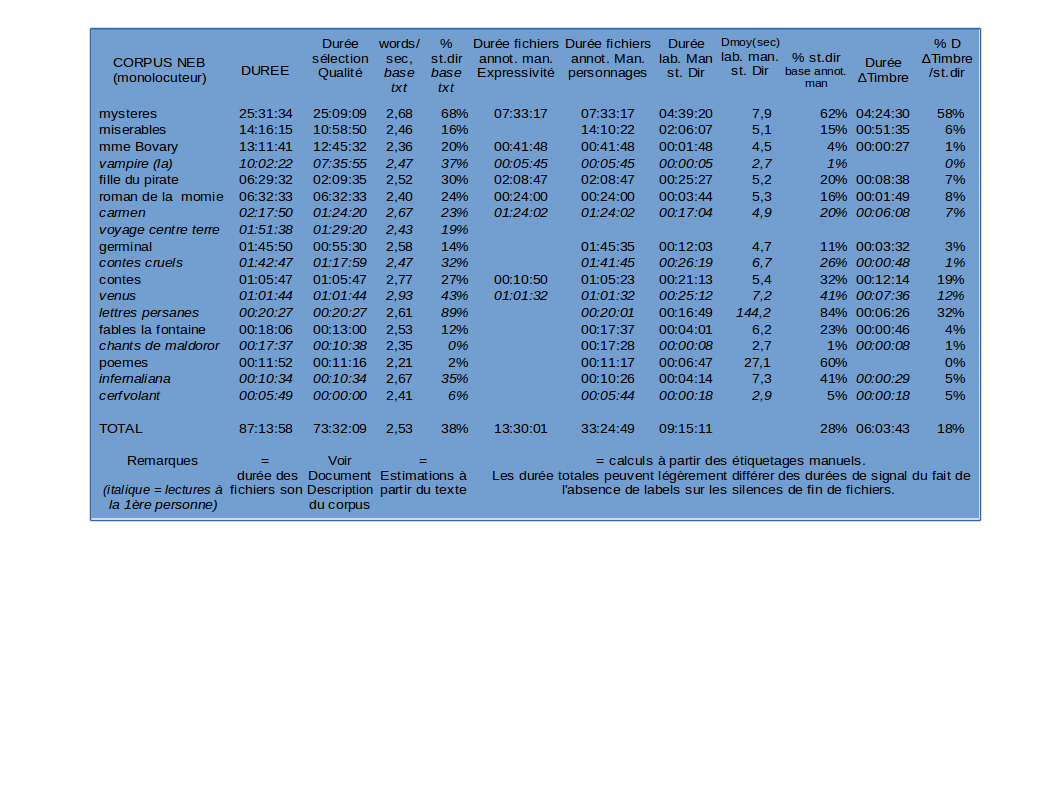
\includegraphics[scale=0.4]{/home/asini/Workspace/TexTemplates/asImages/neb_corpus_gael.png}

\end{figure}

\end{frame}
%============================================================%
%
%============================================================%
\section{Prosody}
\subsection{Prosody Modeling}
\begin{frame}{Some Related Work}
	
\end{frame}

\subsection{Prosody Prediction}
\begin{frame}{Some Related Work}
	
\end{frame}
%============================================================%
%
%============================================================%

\subsection{Raised Questions?}
\begin{frame}{Questions?}

\end{frame}

\section{Summary}
\subsection{Future scope of work}
\begin{frame}{Suggested problems to work on}
	\begin{itemize}
		\item direct and indirect  discourse.
	\end{itemize}
\end{frame}
\subsection{Work Plan(Schudele)}
\begin{frame}{\textbf{Planning the unplannable?}}
\begin{center}
\begin{figure}
	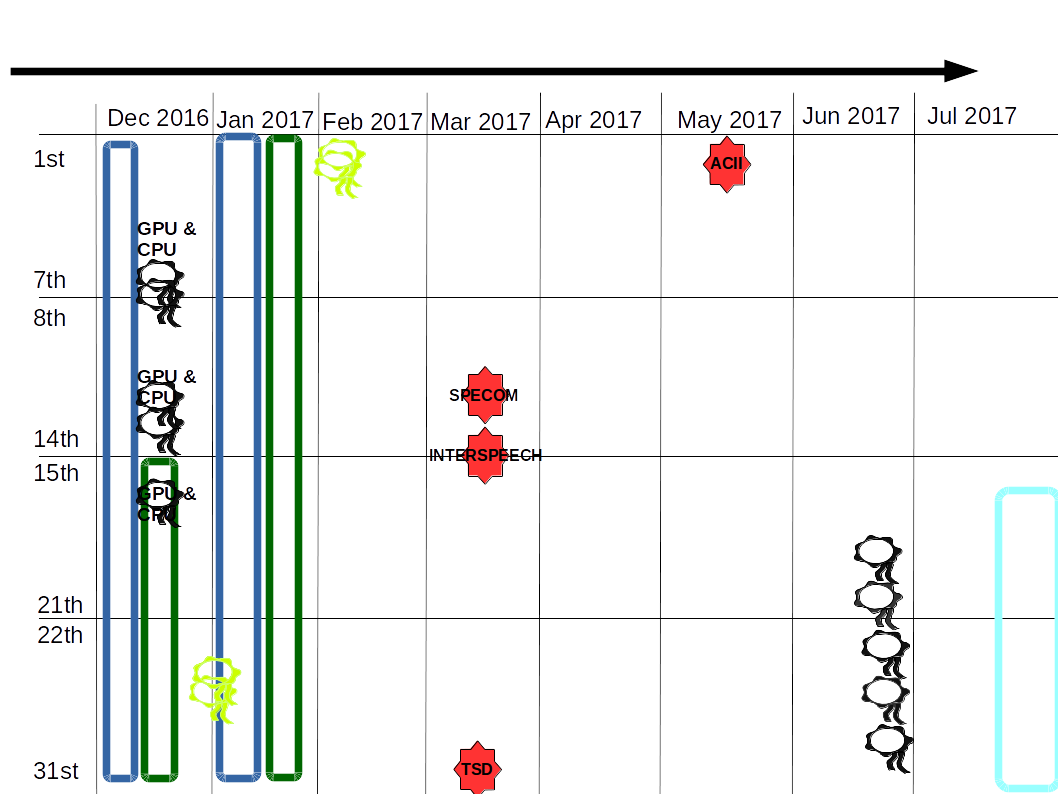
\includegraphics[scale=0.34]{/home/asini/Workspace/TexTemplates/asImages/timeline_schudeler_thesis.png}
\end{figure}
\end{center}
\end{frame}

\begin{frame}
\centering \LARGE THANKYOU
\end{frame}

\subsection{References}
\begin{frame}{References}
\begin{itemize}
	\item Simon, Anne-Catherine; Auchlin, Antoine; Avanzi, Mathieu \& Goldman, Jean-Philippe. Les phonostyles: une description prosodique des styles de parole en français, Rev. Abecassi, M. \& G. Ledegen, Les voix des Français. En parlant, en écrivant, Peter Lang ,\textbf{2010}, 71-88

\item Sandrine, Brognaux; Thomas, Drugman \& Marco, Saerens. Synthesizing Sports Commentaries: One or Several Emphatic Stresses? Rev. Nick Campbell, Dafydd Gibbon \& Daniel Hirst (eds.), Social and Linguistic Speech Prosody. Proceedings of the 7th international conference on Speech Prosody, \textbf{2014}, 270-274

\item Brognaux, Sandrine; Picart, Benjamin \& Drugman, Thomas. Synthèse de commentaires sportifs: intégration d’une annotation prosodique à deux niveaux dans un synthétiseur HMM. Rev. Nouveaux Cahiers de la Linguistique Française.
\textbf{2014}, 31, 335.

\end{itemize}
\end{frame}

\begin{frame}{References (Continued)}
\begin{itemize}
  \ite Rajeswari; K C \& Uma; Maheswari; P. Prosody Modeling Techniques for Text-to-Speech Synthesis Systems ? A Survey,J.     International Journal of Computer Applications,
	\textbf{2012}, 39, 16, 8-11.

  \item Silverstein, K. A. T.; Haymet, A. J. D.; Dill, K. A. Molecular Model of Hydrophobic Solvation J. Chem. Phys. \textbf{1999}, 111(17), 8000-8009 
\end{itemize}
\end{frame}


\end{document}
